 %!TeX root = PHYS42 Lecture Notes.tex
\documentclass{article}
\usepackage[dvipsnames, svgnames, x11names]{xcolor}
\usepackage{tikz}
\usepackage{pgfplots}
\usepackage{pgfplotstable}
\usepackage{setspace}
\usepackage{units}
\usepackage{booktabs}
\usepackage{graphicx}
\usepackage{amsfonts}
\usepackage{mathrsfs}
\usepackage{circuitikz}
\usepackage{multirow}
\usepackage{amsopn}
\usepackage{bbding}
\usepackage{amsmath}
\usepackage{hyperref}
\usepackage{cancel}
\usepackage{gensymb}
\usepackage[margin = 1.2in]{geometry}
\newcommand{\RA}{\Rightarrow}
\newcommand{\ra}{\rightarrow}
\newcommand{\dydx}{\frac{dy}{dx}}
\newcommand{\dxdy}{\frac{dx}{dy}}
\newcommand{\midlabelline}[3]{
   \node (midlabel) at ($ (#1)!.5!(#2) $) {#3};
   \draw[latex-] (#1) --  (midlabel);
   \draw[-latex] (midlabel) -- (#2);
}

\AtBeginEnvironment{document}{\everymath{\displaystyle}}
\title{MATH 2 Lecture Notes}
\date{Tuesday, 14 January, 2025}
\author{Tejas Patel}
\begin{document}
\maketitle
\tableofcontents
\pagebreak
\section{Chapter 1}
\subsection{Terminology}
\textbf{Definition} A differential equation is an equation containing the derivatives or differentials 
of one or more dependent variables, with respect to one or more independent variables.\\
\textbf{$\cdot$} An Ordinary Differential Equation (ODE) involves only ordinary derivatives\\
\textbf{$\cdot$} A Partial Differential Equation (PDE) involves partial derivatives.\\
\textbf{Definition} The order of a DE is the order of the highest-order derivative that appears in the DE
\textbf{Notation} $F(x,y,\frac{dy}{dx}, \frac{d^2y}{dx^2})$\\
\textbf{Definition} A linear DE is any DE that can be written in form:\\
${\displaystyle a_{0}(x)y+a_{1}(x)y'+a_{2}(x)y''\cdots +a_{n}(x)y^{(n)}=b(x)}$\\
For a DE to be linear:
\begin{enumerate}
    \item Y and all of its derivatives much be of the 1st degree
    \item Any term that does not include y or any of its derivatives must be a function of x
\end{enumerate}
\subsection{Some Mathematical Models}
\subsubsection*{I. Free-falling body}
Goal: Find s(t). 
\\Set up a differential equation in S, model it, then solve
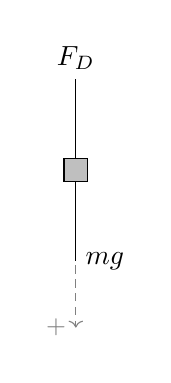
\begin{tikzpicture}[
    force/.style={>=latex,draw=blue,fill=blue},
    axis/.style={densely dashed,gray,font=\small},
    M/.style={rectangle,draw,fill=lightgray,minimum size=0.5cm,thin},
    m/.style={rectangle,draw=black,fill=lightgray,minimum size=0.3cm,thin},
    plane/.style={draw=black,fill=blue!10},
    string/.style={draw=red, thick},
    pulley/.style={thick},
]
\matrix[column sep=1cm] {
    \node[m] (m) {};

    \draw[axis,->] (m) -- ++(0,-2) node[left] {$+$};
    {[force,->]
    \draw (m.north) -- ++(0,1) node[above] {$F_D$};
        \draw (m.south) -- ++(0,-1) node[right] {$mg$};
    }
\\
};
\end{tikzpicture}\\
$ma=mg\\\frac{d^2s}{dt^2}=g\\v=\frac{ds}{dt}, g=\frac{dv}{dt}$\\
What if there is air resistance. Assume force scales linear with velocity
\\$\frac{dv}{dt}=g-\frac{kv}{m} \rightarrow \frac{dv}{dt}=g-\frac{k}{m}\cdot \frac{ds}{dt}$
\subsubsection*{II: Series Circuit}
\begin{circuitikz}
    \draw[line width=0.8]
     (2,7) to [sinusoidal voltage source, l_=$V_S$, i=$I$] (2,1)
     (2,7) to [resistor, l_=$R$] ++(6,0) to [inductor, l_=$L$] ++(0,-6) to [capacitor, l_=$C$] +(-6,0) ;
    \midlabelline{2,8}{8,8}{$V_R$}
    \midlabelline{9,7}{9,1}{$V_L$}
    \midlabelline{2,0}{8,0}{$V_C$}
\end{circuitikz}

Voltage drops:\\ $
V=L \frac{dI}{dt}, V=L \frac{d^2q}{dt^2}\\
V=IR, V= R \frac{dq}{dt}\\
V=\frac{q}{C}\\
E(t) = L \frac{d^2q}{dt^2}+ R \frac{dq}{dt} + \frac{q}{C}
$
\subsubsection*{III: Population Growth}
$P=P(t) =$ population at time t — use exponential model \\
$\frac{dp}{dt} \propto P \rightarrow \frac{dp}{dt} = kP \rightarrow = Ce^{kt}$ where C is the initial population
\subsubsection*{IV: Population Growth with Finite Capacity}
"Carrying Capacity" = N — uses the logistic growth model\\
$\frac{dp}{dt} \propto $ both P and amount to carrying capacity (N-P)\\
$\frac{dp}{dt}=kP(N-P)$
\subsubsection*{V: Chemical Reaction}
$A+B\rightarrow C$ Concentrations of A and B decreases by amount of C formed \\ 
Can we write DE governing the concentration of C x(t)? \\ 
The rate at which the reaaction takes place $\propto$ Product of the remaining concentrations of A and B
\\ $\alpha$ initial concentration of A
\\ $\beta$ initial concentration of B
\\ $\frac{dx}{dt} = k(\alpha - x)(\beta - x)$
\section{First-Order Differential Equations}
\subsection{Preliminary Theory}
Example DE: $y'=3y \Rightarrow \boxed{y=Ce^{3x}}$ the general solution where C is an arbitrary constant
\\[0.05in]Add initial condition $y(0) = 5$ plug in x=0 to $5=Ce^{3*0}, 5=C*1, C=5 \Leftarrow$ Initial Value Problem
\\$y=5e^{3x}$ is the general solution for the Initial Value Problem\\\subsubsection{\textbf{Theorem}}
$f(x) = \begin{cases}
    \frac{dy}{dx} = f(x,y) & \text{Differential Equation}\\
    y(x_0) = y_0  & \text{Initial Condition}
    \end{cases}$\\ Let R be a rectangular region in the xy-plane defined by $a\leq x \leq b, c \leq y \leq d $, that contains the point $(x_0, y_0)$ in its interior. \\[0.1in] If f(x,y) and $\frac{\partial f}{\partial y}$ are continuous on $R$, then there exists an interval I centered at $x_o$, and on this interval $I$ there exists a unique solution $y(x)$ for this IVP\\
\subsubsection{\textbf{Key Questions:}}Does every IVP have at least one solution?\\ If an IVP has a solution is it the only solution?

\textbf{Meaning of a solution existing "on an Interval"}
The initial value problem
\\$\begin{cases}
    \frac{dy}{dx} =1+y^2
    \\ y(0)=0
\end{cases}$ has a unique solution. In fact, we can easily verify that $y=\tan x$ satisfies this IVP
\\ However note that there are some inervals on which $y=\tan x$ cannot be a solution for this IVP, such as (-2,2),
where the function is discontinuous at $\pm \frac{\pi}{2}$ but can be used for (-1,1) since it is continuous at all points within the interval
\subsection{Separable Variables (Separable Equations)}
\subsubsection{\textbf{Definition: }}A differential equation that can be written in the form $\frac{dy}{dx}= \frac{g(x)}{h(y)}$ is said to be separable (or have separable variables).
\\\textbf{Example: } $\frac{dy}{dx}= \frac{g(x)}{h(y)} \\[0.05in]h(y) dy = g(x) dx \\[0.05in] \int{h(y)}{dy} = \int g(x) dx$ 
\\\textbf{Example: } $dx+e^{3x}dy=0$ \\ $e^{3x} dy = -dx$ \\ $dy=-\frac{dx}{e^{3x}}\rightarrow dy=-{e^{-3x}}{dx} \rightarrow \int dy=\int -{e^{-3x}}{dx} \rightarrow y=\frac{1}{3}e^{-3x}+C$ where C is an arbitrary constant
\subsubsection{Substitution} $\frac{dy}{dx} = F(ax+bc+c)$ where $b\neq 0$ use the substitution: $u=ax+by+c \Rightarrow \frac{du}{dx} = a+b\frac{dy}{dx} = \frac{1}{b}\left[\frac{du}{dx}-a\right]$
\\Example: $\frac{dy}{dx} = \tan^2(x+y)$ let $u=x+y \rightarrow \frac{dy}{dx}=\frac{du}{dx}-1 \rightarrow \frac{du}{dx}-1=\tan^2 u \rightarrow \frac{du}{dx} = \sec ^2 u \\ \int \cos^2 u \; du = \int dx \\ 2(x+y)+\sin2(x+y) = 4x+C \rightarrow 2y-2x+\sin2(x+y)$
\\ \textbf{Solve:}
$\frac{dy}{dx} = (y+3)^2$ By inspection $y=-3$ is a solution. This is the only solution because $f(x,y)=(x+3)^2$ is continuous on $\mathbb{R}^2$ and $\frac{\partial f}{\partial x}$ is continuous on$ \mathbb{R}$ so it is the only solution
Why solving by separation is not possible
$\int (y+3)^-2 dy=\int dx \rightarrow (y+3)^-2/-1=x+C_1 \rightarrow \frac{1}{y+3}=-x-C_1 \rightarrow y+3 = \frac{1}{c-x} \rightarrow y=-3+\frac{1}{c-x}
\\y(0)=-3\rightarrow 0=\frac{1}{c}$ where there is no real c that solves that equation, making this not possible
\subsection{Homogeneous Equations} 
\textbf{What do we do if the DE is not separable?}
\subsubsection{Definition} A function $f(x,y)$ is said to be \textbf{homogeneous of degree} $n$ if, for $x, y,$ and$ t $where $f(x,y)$ and $f(tx,ty)$ are defined: \\$$f(tx,ty)=t^nf(x,y)$$
\subsubsection{Example} Determine wheteher each function is homogeneous: \\
a: $ f(x,y)=x^3-7x^2y+4y^3 \rightarrow f(tx,ty)=(tx^3)-7(tx)^2(ty)+4(ty)^3\\t^3x^3-7t^3x^2y+4t^3y^3\\t^3(x^3-7x^2y-4y^3)=t^3f(x,y)$
\\How to tell quickly wheteher $f(x,y)$ is homogeneous:
\\Each term must have the same combined degree
\\Example: $x^3-7x^2y+4y^3$ is D3, $x^2+y^2-4x$ is not, $\sqrt{x^5+4y^5}$ is with D 2.5, $\frac{3y}{x}-2$ is D0
\subsubsection{Differential Equation form}
$M(x,y)dx+N(x,y)dy=0$ is called a homogeneous differential equation if the functions $M$ and $N$ are both homogeneous of the same degree
\\If $f(x,y)$ is homogeneous of degree $n$ then $f(x,y)$ can be written as:
\\$f(x,y)=f\left(x\times 1, x \times \frac{y}{x}\right)=x^nf\left(1, \frac{y}{x}\right)$
\\or $f(x,y)=y^nf\left(\frac{x}{y},1\right)$
\subsubsection{Substitution} To solve a homogeneous DE make the substitution: $y=ux \;\; (u=\frac{y}{x})$ or$ x=vy \; \; (v=\frac{x}{y})$
\subsubsection{Example}
$(y^2+xy)dx+x^2dy=0 \rightarrow y=ux \rightarrow dy=(udx+xdu) \\ (u^2x^2+ux^2)dx+x^2(udx+xdu)=0\\u^2x^2dx+ux^2dx+ux^2dx+x^3du=0 \\ ux^2(u+2)dx+x^3du=0\\\int \frac{1}{u(u+2)}du=-\int \frac{1}{x}dx \\$ Partial Fraction Decomposition: $\frac{1}{u(u+2)}=\frac{A}{u}+\frac{B}{u+2} \rightarrow A=\frac{1}{2}, B=-\frac{1}{2}$ Back to solving \\ $\int \left[\frac{0.5}{u}-\frac{0.5}{u+2}\right]=-\int \frac{1}{x} dx \\ 0.5\ln|u|-1/2 \ln |u+2|=-\ln |x|+C_1 \\ \ln \left|\frac{u}{u+2}\right|=2C_1-2\ln|x| \\ \left|\frac{u}{u+2}\right|=e^{2C_1}\cdot e^{-2\ln|x|} = e^{2C_1}\cdot |x^{-2}| \Rightarrow \left|\frac{u}{u+2}\right| = \left|e^{2C_1}\cdot x^{-2}\right| \Rightarrow \left|\frac{u}{u+2} = \frac{C}{x^2}\right| \\ ux^2=X(u+2) \Rightarrow ux^2=Cu+2c \rightarrow ux^2-Cu=2C \\ u(x^2-c)=2C \Rightarrow u= \frac{2C}{x^2-C} \Rightarrow \frac{y}{x} = \frac{2Cx}{x^2-C}, \; x \neq 0$
\subsection{Exact Equations}
Recall from Math 1C: Let $F(x,y)=\langle 3x^2-7y, -7x+2y \rangle$
\begin{enumerate}
    \item If F a conservative vector field 
    \\i.e., Is there a function $f(x,y)$ such that $\nabla f$? Yes, -7=-7
    \item If F is indeed conservative, what is f? \\ $x^3-7xy+g(y)=f(x,y)\\-7x+2y, g'(y)=2y \\ f(x,y)=x^3-7xy+y^2+k$
\end{enumerate}
\subsubsection{Definition} A differential equation in the form $M(x,y)dx+N(x,y)dy=0$ where $M_y=N_x$, is called an exact differential equation.
\subsubsection{Solve the DE}
$(3x^2-7y)dx+(-7x+2y)dy=0$ \\Using 1C techniques it is $f(x,y)=x^3-2xy+y^2+k$
\\Set this f = c. $f(x,y)=x^3-2xy+y^2=c$ take k=0 in every problem
\\If the DE is not exact, sometimes we can make it exact by multiplying by magical quantity $\mu (x,y)$
\subsubsection{Example:} Solve the DE:
\\$(x+y)dx+xlnxdy=0$ using $\mu(x,y)=\frac{1}{x}$
\\$\left(\frac{x+y}{x}\right)dx+\ln|x|\;dy=0$ is now exact.
\\Solution: $f(x,y)=x+y\ln x=c$
\subsection{Linear Equations}
Recall: First Order Linear DE is a DE in the form $a_1(x)\frac{dy}{dx}+a_0(y)y=g(x),\qquad a_1(x)\neq 0$
\\Divide both sidex by $a_1(x) \Rightarrow \frac{dy}{dx}+\frac{a_0(x)}{a_1(x)}y=\frac{g(x)}{a_1(x)}$ where $P(x)=\frac{a_0(x)}{a_1(x)}$ and $f(x)=\frac{g(x)}{a_1(x)}$\\
\\$\frac{dy}{dx}+P(x)y=f(x)$ There is an integrating factor $\mu(x)$ that turns this DE into an exact DE
\\$dy+P(x)ydx=f(x)dx \rightarrow dy\left[P(x)y-f(x)\right] dx=0 
\\\mu(x)dy+\mu(x)\left[P(x)y-f(x)\right]dx=0 \rightarrow \mu '(x)=\mu(x)P(x) \\ \frac{d\mu}{dx}=\mu P
\rightarrow\int \frac{d\mu}{mu}=\int P(x)\rightarrow\ln\mu=\int P(x)\; dx
\\\mu(x)=e^{\int P(x)\; dx} \Rightarrow e^{\int P(x)\; dx} \frac{dy}{dx}+ e^{\int P(x)\; dx} P(x)y=e^{\int P(x)\; dx}f(x)
\\\frac{d}{dx}\left[e^{\int P(x)dx}y\right]=e^{\int P(x)dx}f(x) \rightarrow e^{\int P(x)dx}y=\int e^{\int P(x)dx}f(x)dx$
\boxed{y=e^{-\int P(x)dx}\int e^{\int P(x)dx}f(x) dx}
\subsubsection{Procedure to follow for every Linear DE}
\begin{enumerate}
    \item Rewrite the linear DE in the form $\frac{dy}{dx}+P(x)y=f(x)$
    \item Find the integrating factor $\mu(x)=e^{\int P(x)dx}$
    \item Multiply each side of the DE by $\mu(x)$
    \item Rewrite the left side as $\frac{d}{dx} \left[\mu(x)\cdot y\right]$
    \item Integrate both sides with respect to x and retreive an implicitly expressed solution
    \item Solve for y
\end{enumerate}
\subsection{What method to use to solve?}
First ask is it exact? $(M_y=M_x)$
\\Yes: Use the method in $\S$2.4
\\No: Is it linear? (in y or x)
\\Yes: Use the method in $\S$2.5
\\No: Is it separable?
\\Yes: $\S 2.2$
\\No: Homogeneous?
\\Yes: Use a substitution $\S 2.3$
\\No: Good luck. or use inspection\pagebreak
\section{Applications of First-Order Differential Equation}
\subsection{Orthogonal Trajectories}
$\cdot$ Consider the family of curves $y=cx^3$
Question: Which DE should be solved to get this family as its solutions?
\\Steps:
\begin{enumerate}
    \item Find $\frac{dy}{dx} =3cx^2$
    \item Eliminate c"
\end{enumerate} $y=cx^3 c=\frac{y}{x^3} \\ \frac{dy}{dx}=3\frac{y}{x^3}x^2 \rightarrow \frac{3y}{x}$

\textbf{$\cdot$} The two curves are orthogonal if their tangent lines are orthogonal at the point of intersection
\\i.e. The derivatives are the negative reciprocals of each other
\subsubsection{Example}
Show that $y=x^3$ and $x^2+3y^2=4$ are orthogonal at their points of intersection, (1,1) and (-1,-1)
\\ $y=x^3 \Rightarrow \frac{dy}{dx}=3x^2 \rightarrow =3$ at $x=1$ and 3 at $x=-1$
\\$2x+6y\frac{dy}{dx}=0 \rightarrow \frac{dy}{dx}=-\frac{x}{3y} = \frac{-1}{3}$ at both $x=1$ and $x=-1$ meaning it is orthogonal
\subsubsection{Definition} When all the curves of one family of curves intersect orthogonally all the curves of another family, then the families are said to be orthogonal trajectories of each other
\subsection{Applications of Linear Equations}
$\frac{dN}{dt}=kN\rightarrow N=Ce^{kt}$ for bacterial growth rate. Nothing else here, just an applications section
\subsection{Applications of Nonlinear Equations}
\subsubsection*{Logistic Model of Population Growth}
1: End Behaviour (Steady State Solution)
as $t\rightarrow \infty P(t)=\frac{aP_0}{bP_0+(a-bP_0)e^{-at}} \rightarrow P(t)=\frac{aP_0}{bP_0}=\frac{a}{b}$
2: Concavity Analysis (Point of Inflection)
$\frac{dP}{dt}=P(a-bP)\\\frac{d^2P}{dt^2}=\frac{dP}{dt}(a-2bP)=P(a-bP)(a-2bP)=0$ \\ For inflection point $a-2bP=0\rightarrow a=2bP \rightarrow P=\frac{a}{2b} \rightarrow P=\frac{N}{2}$
3 cases of initial conditions
$\begin{cases}
    0<P_0<\frac{a}{2b} & \text{Hits inflection point while rising to CC}\\
    \frac{a}{2b}<P_0<\frac{a}{b} & \text{Population grows at a decreasing rate to CC}\\
    P_0>\frac{a}{b} & \text{Population falls to the carying capacity}
\end{cases}$
\section{Linear DE of Higher Order}
\subsection{Preliminary Theory}
Initial Value Problem $a_n(x)y^{(n)}+a_{n-1}(x)y^{(n-1)}+...+a_1(x)y'+a_0(x)y=g(x)$
\\Initial Conditions $y(x_0)=y_0...y^{(n-1)}(x_0)=y_0^{(n-1)}$
\\\textbf{Theorem} Let easch $a_j(x)$ be continuous on an interval I and let $a_n(x)\neq 0$ for every... CONTINUE LATER
\\Boundary-Value Problem for 2nd order Linear DE $a_2(x)y''+a_1(x)y'+a_0(x)y=g(x)\\  \qquad y(a)=y_0 \qquad y(b)=y_1$
\\Example: $y''+16y=0 \quad y(0)=0 \quad y(\pi/2) = 0
\\y=\sin 4x$ and $y=\cos 4x$ are solutions so $y(x)=c_1\cos 4x+ c_2 \sin 4x
\\y(0) = c_1\cos(0)+c_2\sin(0) =c_1= 0
\\y(\pi/2) = c_1\cos(2\pi)+c_2\sin(2\pi) =c_1= 0
$ so $y(x)=c_2\sin 4x$ is a solution

\subsection{Constructing a Second Solution from a Known Solution}

\subsubsection*{General Formula} Given $a_2(x)y''+a_1(x)y'+a_0(x)y=0$ and $a_2(x) \neq 0$ and $y_1(x) \neq 0$ is a solution of this DE, find $y_2(x)$
\\Divide by $a_2(x)$: $y''+\cancelto{P(x)}{\frac{a_1(x)}{a_2(x)}}y'+\cancelto{Q(x)}{\frac{a_0(x)}{a_2(x)}}y=0
\\y''+Py'+Qy=0, \quad y_2=uy_1 \rightarrow y_2'=uy'1+u'y_1 \rightarrow y_2''=uy_1''+2u'y_1'+u''y_1$ 
\\Plug it all in: $u''y_1+2u'y_1'+uy_1''+Py'y_1+Puy_1'+Quy_1=0
\\u''y_1+u'(2y_1'+Py_1)+\cancelto{0}{u(y_1''+Py_1'+Qy_1)}=0
\\u''y_1+u'(2y_1'+Py_1)=0$ Let w=u' and w'=u''
\\$y_1w'+(2y_1'+Py_1)w=0
\\ w'+\frac{2y_1'+Py_1}{y_1}w=0 \quad \mu = e^{\int \frac{2y_1'}{y_1}+P dx}
\\w=c_1y_1^{-2}e^{-\int P dx}=u' = {e^{-\int P dx}}{y_1^2}$
\\\subsubsection{General Reduction of Order Formula} $y=C_1y_1+C_2y_2$ where \boxed{y_2=y_1\int \frac{e^{-\int P dx}}{{y_1^2}} dx}


\subsection{Homogeneous Linear Equations w/ Constant Coefficients}
In the DE $a_2(x)y''+a_1(x)y'+a_0(x)y=0$, take \\
$a_2(x)=a,\qquad a_1(x)=b,\qquad a_0(x)=c$
\\ so we have a 2ns-order Homogeneous Linear DE with \textit{constant coefficients}
$$ay''+by'+cy$$
\\What does a typical solution look like?
\\$\begin{cases}
    y=e^{mx}
    \\y'=me^{mx}
    \\y''=m^2e^{mx}
\end{cases}$ so $am^2e^{mx}+bme^{mx}+ce^{mx}=0=e^{mx}(am^2+bc+c)$
\subsubsection{Auxilliary Equation for a DE} $am^2+bm+c=0$
\subsubsection{Three Scenarios for the Auxilliary Equation}
$\begin{cases}
    \text{If}\;\; b^2-4ac>0 & \text{two real roots}\;\; y=c_1e^{m_1x}+c_2e^{m_2x}
    \\ \text{If}\;\; b^2-4ac=0 & \text{one real root}\;\; y=c_1e^{mx}+c_2xe^{mx}
    \\\text{If}\;\; b^2-4ac<0 & \text{No real roots, 2 distinct complex roots}, y=e^{\alpha x}\left(C_1\cos \beta t +C_2\sin \beta t\right)\; m=\alpha \pm i\beta
\end{cases}$
\subsection{Undetermined Coefficients - Superposition Approach}
$\bullet$ Nonhomogeneous Linear DE with constant coefficients:
$$ay''+by'+cy=g(x)$$
\textbf{Recall from Section 4.1}: The general solution is: $$y(x)=y_c(x)+y_p(x)$$ where $y_c(x)$ is the general solution $ay''+by'+cy=0$\\ $y_p(x)$ is one particular colution of $ay''+by'+cy=g(x)$
\\\textbf{The big question:} How do we find $y_p(x)$?
\subsubsection{Trial Particular Solutions} 
\begin{tabular}{|c|c|}
    g(x) & Form of $y_p$
    \\constant & $A$
    \\ $2x-7$ & $Ax+B$
    \\$-x^2+3$& $Ax^2+Bx+C$
    \\ $\sin kx$ or $\cos kx$ & $A \cos kx + B \sin kx$
    \\ $e^{kx}$ & $Ae^{kx}$
    \\$(2x-7)e^{kx}$ & $(Ax+B)e^{kx}$
    \\$x^2e^{kx}$ & $(Ax^2+Bx+C)e^{kx}$
    \\$ e^{kx} \cos lx$ $or e^{kx} \sin lx$ & $e^{kx}(A\cos lx + B \sin lx)$
    \\ $5x^2 \sin kx$ & $(Ax^2+Bx+C)\cos kx + (Dx^2+Ex+F)\sin kx$
    \\ $xe^{kx} \cos lx$ & $(Ax+B)e^{kx}\cos lx + (Cx+D)e^{kx}\sin lx$
\end{tabular}
\subsection{Variation of Parameters}
Given: $a_2(x)y''+a_1(x)y'+a_0(x)y=g(x)\\\Rightarrow y''+P(x)y'+Q(x)y=f(x)$
\\Goal: Find $y_p$
\subsubsection{Idea:} Let $y_1,\;y_2$ be the two linearly independent solutions of $$y''+P(x)y'+Q(x)y=0$$ Then we will look for $y_p$ of the form: $$y_p=u_1(x)y_1(x)+u_2(x)y_2(x)$$
\subsubsection{Derivation:} $y_p'=u_1'y_1+u_2'y_2+u_1y_1'+u_2y_2'$ by product rule \\[0.1in] Assume $u_1'y_1+u_2'y_2=0 \rightarrow y_p'=u_1y_1'+u_2y_2'$
\\[0.1in]$y_p''=u_1y_1''+u_2y_2''+u_1'y_1'+u_2'+y_2'$ then substitute into  $y''+Py'+Qy=f$
\\[0.1in] $\cancelto{0}{u_1(y_1''+Py_1'+Qy_1)}+\cancelto{0}{u_2(y_2''+Py_2'+Qy_2)}+u_1'y_1'+u_2'+y_2'=f$
\\[0.1in]$\begin{cases}
    u_1'y_1+u_2'y_2=0
    \\u_1'y_1'+u_2'+y_2'=f
\end{cases} \rightarrow y_p=u_1y_1+u_2y_2$ 
\subsubsection{Example}$y''+9y=\cos 3x$
\\[0.1in]$m^2+9=0 \rightarrow m=\pm 3i \rightarrow y_c=C_1 \cos 3x + C_2 \sin 3x $
\\[0.1in]$y_p=u_1y_1+u_2y_2$ where $u_1'=\frac{\begin{bmatrix}0&\sin 3x\\\cos 3x&3\cos 3x\end{bmatrix}}{\begin{bmatrix}\cos 3x&\sin 3x\\3\sin 3x & 3\cos 3x \end{bmatrix}}= -\frac{1}{3}\sin 3x \cos 3x = -\frac{1}{6}\sin 6x\\
u_1=\int -\frac{1}{6}\sin 6x dx = \frac{\cos 6x}{36}$\\
$u_2'=\frac{\begin{bmatrix}\cos 3x & 0 \\ -3\sin 3x & \cos 3x\end{bmatrix}}{\begin{bmatrix}\cos 3x&\sin 3x\\3\sin 3x & 3\cos 3x \end{bmatrix}} = \frac{\cos^2 3x}{3}=\int \frac{\cos^2 3x}{3} dx=\int \frac{1+ \cos 6x}{6} dx = \frac{x}{6}+\frac{\sin 6x}{36}$
\\$y_p=\frac{\cos 6x }{36}\cos 3x + \frac{x}{6}+\frac{\sin 6x}{36}\sin 3x = \frac{1}{36}\cos 3x + \frac{x}{6}\sin 3x$
\\$y_p=C_1 \cos 3x + C_2 \sin 3x+\frac{1}{36}\cos 3x + \frac{x}{6}\sin 3x =$ \boxed{C_1\cos 3x + C_2 \sin 3x + \frac{1}{6}x \sin 3x}\\
\textbf{Initial Value Problem} $y(0)=1,\quad y'(0)=0$
\\$C_1\cos 3x + \cancelto{0}{C_2 \sin 3x + \frac{1}{6}x \sin 3x} \rightarrow C_1 \cos(0)=1 \rightarrow C_1=1$
\\$y'(0) \rightarrow \cancelto{0}{-3\sin 3x} +3C_2\cos 3x+\frac{1}{6}x+3\cos 3x + \cancelto{0}{\frac{1}{6}\sin 3x}\\
3C_2\cos 3x+\frac{1}{6}x+3\cos 3x=0 \rightarrow 3C_2=0$ so $C_2=0$
\\\boxed{y(x) = \cos 3x + \frac{1}{6}x \sin 3x}
\pagebreak
\section{Applications of 2nd-Order DE}
\subsection{Simple Harmonic Motion}
$\frac{d^2x}{dt^2}+\omega ^2s=0$ where $\omega = \sqrt{\frac{k}{m}}$
\\Auxilliary Equation: $m^2\omega ^2=0 \quad m=0\pm\beta i$
\\$C_1cos \omega t + C_3 \sin \omega t = A\sin (\omega t + \phi)$ where $A=\sqrt{C_1^2+C_2^2},\;\; \sin\phi=\frac{C_2}{A},\;\; \cos\phi=\frac{C_2}{A},\;\;\tan\phi=\frac{C_1}{C_2}$
\subsubsection{Example}
A 16lb weight is attached to a spring, stretching it 1.28 feet. This weight is released 2 feet above the equilibrium position, with initial downward velocity of 1.5 ft/s
\\DE: $m\frac{d^2x}{dt^2}+kx=0$
$\begin{cases}
    \text{Weight}&w=mg=\frac{1}{2} \text{Slug}
    \\k&F=k\cdot s = 16=k*1.28,\quad 12.5 \frac{lb}{ft}
\end{cases}$
\\$\frac{d^2x}{dt^2}+25x=0,\quad x(0)=-2,\quad x'(0)=-1.5$
\\Solve the equation: $x(t)=C_1\cos 5t +C_2\sin 5t $
\\$x(t)=-2\cos 5t + 0.3\sin 5t$
\\Period is $\frac{2\pi}{5}$ seconds or $\frac{5}{2\pi}$ vps
\subsection{Damped Motion}
\subsubsection{Differential Equation form}
$\frac{d^2x}{dt^2}+2\lambda \frac{dx}{dt}+\omega ^2 x=0$
Forms of solutions
\subsection{Forced Motion}
With the presence of an external force, the equation of motion has another extra term:
\\$x \frac{d^2x}{dt^2}=-kx-\beta \frac{dx}{dt}+f(t)$ where $k>0$
\subsubsection{Example}
8lb weight, 32/13 ft stretch when hung freely, starts 3 feet below equilibrium, find equation of motion if $f(t)=18.75\sin 2t$ is applied and damping force is 1.5x instantaneous velocity
\\$m \frac{d^2x}{dt^2}+\beta \frac{dx}{dt}+kx=f(t)
\\m=\frac{1}{4} , ~\beta = 1.5 ~ k:8=k\cdot\frac{32}{13}=\frac{13}{4}
\\ \frac{1}{4}x''+\frac{6}{4}x'+\frac{13}{4}x=18.75\sin 2t
\\x''+6x'+13x=75\sin 2t ~ x(0)=3~x'(0)=0 \\ x_p=A\cos 2t+B\sin 2t ~ A=-4, ~ B=3
\\x(t)=c_1e^{-3t}\cos 2t +c_2e^{-3t}\sin 2t-4\cos 2t+3\sin 2t
\\\text{with initial conditions } c_1=7 ~ c_2=\frac{15}{2}
\\x(t)=7e^{-3t}\cos 2t +\frac{15}{2}e^{-3t}\sin 2t-4\cos 2t+3\sin 2t
\\-4\cos 2t+3\sin 2t \text{ is the steady state solution and }\\7e^{-3t}\cos 2t +\frac{15}{2}e^{-3t}\sin 2t \text{ is the transient solution} $

\subsection{Electric Circuits \& Other Analogous Systems}
LRC Circuit: For charge $q=q(t)$ and currtent $i = i(t) = \frac{dq}{dt}$
$$L \frac{d^2q}{dt^2}+R \frac{dq}{dt} + \frac{q}{c} = E(t) $$
\subsubsection{Example}
$L=2H, ~R=8\Omega, ~C=\frac{1}{18}F, ~E(t)=10\sin(t) \;V, ~q(0)=0, ~ i(0)=0$
$2 \frac{d^2q}{dt^2}+8 \frac{dq}{dt} + 18 \frac{q}{c} = 10\sin t\\ = \frac{d^2q}{dt^2}+4 \frac{dq}{dt} + 9 \frac{q}{c} = 5\sin t 
\\\frac{d^2q}{dt^2}+4 \frac{dq}{dt} + 9 \frac{q}{c} = 5\sin t \Rightarrow m^2+4m+9=0 \rightarrow m=-2 \pm \sqrt{5}i
\\q_c(t)=c_1e^{-2t}\cos\sqrt{5}t+c_2e^{-2t}\sin\sqrt{5}t 
\\y_p = -\frac{1}{4}\cos t + \frac{1}{2} \sin t \quad \text{time for initial conditions} \\
c_1=\frac{1}{4} \;\; c_2=0 \Rightarrow$ \boxed{q(t)=c_1e^{-2t}\cos\sqrt{5}t-\frac{1}{4}\cos t + \frac{1}{2} \sin t}
\\Steady state charge: $q=-\frac{1}{4}\cos t + \frac{1}{2} \sin t$
\\Steady state current: $i=\frac{1}{4}\sin t + \frac{1}{2} \cos t$

\section{DE with Variable Coefficients}
\subsection{Cauchy-Euler Equations}
Differential Equations of the form:
$$a_nx^ny^{(n)}+a_{n-1}x^{n-1}y^{(n-1)}+...+a_1xy'+a_0y=g(x)$$
\\These are considered equidimensional, where the degree of each monomial coefficient function equals the order of the derivative of y in each term

\subsubsection{General Formula for the Auxilliary Equation}
$am(m-1)+bm+c=0$ is equivalent to $am^2+(b-a)m+c=0$
\subsubsection{Forms of Solutions}
$\begin{cases}
    \text{Two Real Roots} & y=c_1x^{m_1}+c_2x^{m_2}\\
    \text{One Repeated Real Root} & y=c_1x^{m_1}+c_2x^{m_1}\ln x\\
    \text{Complex Conjugate Roots where } m=\alpha \pm i\beta & y=x^\alpha \left[c_1\cos(\beta \ln x)+c_2 \sin(\beta \ln x)\right]
\end{cases}$
\subsubsection{Example Case 1}
Solve $x^2y''+4xy'-4y=0$
\\Assume $y=x^m \Rightarrow -4y=-4x^m\\y'=mx^{m-1} \Rightarrow 4xy'=4mx^m\\y''=m(m-1)x^{m-2} \Rightarrow x^m
\\x^2y''+4xy'-4y=m(m-1)x^m+4mx^m-4x^m \Rightarrow  [m(m-1)+4m-4]x^m=0
\\m^2-m+4m-4=0$ is the auxilliary equation $m=1,\;\;-4 \Rightarrow y_1=x',\;\;y_2=x^{-4}
\\y=C_1x+C_2x^{-4}$
\subsubsection{Example Case 2}
$$9x^2y''+3xy'+y=0 \Rightarrow a=9,~b=3,~c=1 \Rightarrow  (3m-1)^2 \Rightarrow m=\frac{1}{3}$$
\\$y_1=x^{\frac{1}{3}},~y_2=c_2x^{\frac{1}{3}} \ln x
\\y=x^{\frac{1}{3}}+c_2x^{\frac{1}{3}} \ln x$
\subsubsection{Example Case 3}
Solve the IVP: $x^2y''+3x'y+3y=0 \qquad y(1)=1 \qquad y'(1)=-5$
\\$m^2+2m+3=0 \Rightarrow m=-1\pm \sqrt{2}i
y=x^{\frac{1}{3}}+c_2x^{\frac{1}{3}} \ln x
\\y=x^{-1}\left[c_1\cos(\sqrt{2}\ln x)+c_2\sin(\sqrt{2}\ln x)\right]$
\\Now time to plug in initial conditions 
\\$1=1\left[c_1 \cancelto{1}{\cos 0} + c_2 \cancelto{0}{\sin 0} \right] \Rightarrow c_1=1
\\ y'(x)=x^{-1} \left[-c_1\sin(\sqrt{2}\ln x)\frac{\sqrt{2}}{x} +c_1\frac{\sqrt{2}}{x}\cos(\sqrt{2}\ln x)\right]+x^{-2} \left[c_1\cos(\sqrt{2}\ln x)+c_2\sin(\sqrt{2}\ln x)\right]
\\-5=y'(1) = c_2 \cdot \sqrt{2}-1 \Rightarrow c_2=-2\sqrt{2}
\\y(x)=x^{-1}\left[\cos\left(\sqrt{2}\ln x\right)-2\sqrt{2}\sin\left(\sqrt{2}\ln x\right)\right]$
\subsection{Review of Power Series; Power-Series Solutions}
$f(x)=\sum_{n=0}^{\infty}c_n(x-a)^n$
\subsubsection{Example}
Where does $\sum_{n=1}^{\infty} \frac{x^n}{n^2}$ converge?
\\$L=\lim_{k\to \infty}\left|\frac{\frac{x^{k+1}}{(k+1)^2}}{\frac{x^k}{k^2}}\right|=\lim_{k\to\infty}\left|\frac{x^{k+1}}{x^k}\right|\cdot \left|\frac{k^2}{(k+1)^2}\right|
=|x|\cdot \lim_{k\to\infty}\frac{k^2}{(k+1)^2}$ for x=1 and x=-1 both $\sum_{n=1}^{\infty}\frac{1^n}{n^2}$ and $\sum_{n=1}^{\infty}\frac{-1^n}{n^2}$ converges by the p series test and alternating series test
\pagebreak \subsubsection{Write $\sum_{n=1}^{\infty}2nc_nx^{n-1}+\sum_{n=0}^{\infty}6c_nx^{n+1}$ as one series}
Write it out manually
\\First: $2c_1+4c_2x+6c_3x^2+8c_4x^3+... =2c_1+\sum_{n=2}^{\infty}2nc_nx^{n-1} = k=n-1 \quad 2c_1+\sum_{k=1}^{\infty}2(k+1)c_{k+1}x^k$
\\2nd: $\qquad \quad 6c_0x+6c_1x^2+6c_2x^3 = \sum_{n=0}^{\infty 6c_nx^{n+1}} = ~~{k=n-1} ~~ \sum_{k=1}^{\infty}6c_{k-1}x^k$
\\Combine them: $2c_1+\sum_{k=1}^{\infty} (2(k+1)c_{k+1}+6c_k-1) x^k$
\subsubsection{Use Power Series to solve $y'-2xy=0$}
$y=\sum_{n=0}^{\infty}c_nx^n \qquad y'=\sum_{n=1}^{\infty}nc_nx^{n-1} \qquad 2xy=2x\sum_{n=0}^{\infty}c_nx^n = \sum_{n=0}^{\infty}2c_nx^{n+1}
\\y'-2xy=\sum_{n=1}^{\infty}nc_nx^{n-1}-\sum_{n=0}^{\infty}2c_nx^{n+1}$ Let $k=n-1,\; n=k+1$
\\$y'=c_1+\sum_{k=1}^{\infty}(k+1)c_{k+1}x^k \qquad -2xy=-\sum_{k=1}^{\infty}2c_{k-1}x^k
\\y'-2xy= c_1+\sum_{k=1}^{\infty}(k+1)c_{k+1}x^k-\sum_{k=1}^{\infty}2c_{k-1}x^k =c_1+\sum_{k=1}^{\infty}\left[(k+1)c_{k+1}-2c_{k-1}\right]x^k=0
\\c_1=0, \qquad (k+1)c_{k+1}=-2c_{k+1} \Rightarrow c_{k+1}=\frac{2c_{k-1}}{k+1}$
\\$c_0$ is an arbitrary constant $c_1=0 \qquad c_{k+1}=\frac{2c_{k-1}}{k+1}
\\c_2=c_0 \quad c_3=0 \quad c_4=\frac{1}{2}c_0 \quad c_6=\frac{c_0}{6} \quad c_8=\frac{c_0}{24}
\\\begin{cases}
    0 & \text{If n is odd}
    \\\frac{c_0}{\left(\frac{n}{2}\right)!} & \text{If n is even}
\end{cases} 
\qquad \qquad \text{If } m=\frac{n}{2} \Rightarrow \frac{c_0}{m!}$
\\$\sum_{m=0}^{\infty}\frac{c_0}{m!}x^{2m}=c_0\sum_{m=0}^{\infty}\frac{x^{2m}}{m!}$ which converts to $c_0e^{x^2}$
\subsubsection{$4y''+y=0$}
$y= \sum_{n=0}^{\infty}c_nx^n \qquad y'=\sum_{n=1}^{\infty}nc_nx^{n-1} \qquad y'' = \sum_{n=2}^{\infty}n(n-1)c_nx^{n-2}
\\4y'' = \sum_{n=2}^{\infty}4n(n-1)c_nx^{n-2} \qquad y=\sum_{n=0}^{\infty}c_nx^n \Rightarrow \sum_{k=0}^{\infty}(4(k+2)(k+1)c_{k+2}+c_k)x^k=0
\\\text{Solve for }c_{k+2} = -\frac{c_k}{4(k+1)(k+2)} \;\; k\in \mathbb{Z}
\\c_2=-\frac{c_0}{8} \qquad c_3=\frac{c_1}{24} \qquad c_4=\frac{c_0}{4^2\cdot 4!} \qquad c_5=\frac{c_1}{4^2 \cdot 5!}$
\\[0.05in]General Pattern: $\begin{cases}
    c_n=(-1)^{\frac{n}{2}}\frac{c_0}{4^{\frac{n}{2}}\cdot n!} & \text{ When n is even}
    \\c_n=c_{2m+1} = (-1)^m \cdot \frac{c_1}{4^m\cdot (2m+1)!} & \text{ When n is odd}
\end{cases}
\\ c_0\sum_{m=0}^{\infty} \frac{(-1)^m}{(2m)!}\left(\frac{x}{2}\right)^{2m}+c_1\sum_{m=0}^{\infty}\frac{(-1)^m}{(2m+1)!}\left(\frac{x}{2}\right)^{2m+1}
$ 
\\Converts to $y=c_1\cos\frac{x}{2}+c_2\sin\frac{x}{2}$

\section{Laplace Transformations}
\subsection{Laplace Transform:}
\begin{itemize}
    \item Method used to solve certain DEs in an easier way
    \item Converts DE/IVP into simpler equations
\end{itemize}
\subsubsection{Definition}
Let $f(t)$ be a function, where $t\geq 0$ then $$\mathscr{L}\left\{f(t)\right\}=\int_{0}^{\infty}e^{-st}f(t) dt,~s>0$$
\subsubsection{Example $\mathscr{L}$}
$\int_{0}^{\infty} e^{-st}* 1 dt = \lim_{b\to \infty}\int_{0}^{b}e^{-st} dt = \lim_{b \to \infty} {\left[\frac{e^{-st}}{-s}\right]_{t=0}}^{t=b}$ results in $\frac{1}{s}$
\subsubsection{Theorem}
$\mathscr{L}\left\{\alpha f(t) + \beta g(t)\right\}-\alpha\mathscr{L}\left\{f(t)\right\}+\beta\mathscr{L}\left\{g(t)\right\}$
\subsubsection{Theorem}
If $f$ is piecewise continuous on $[0,\infty)$, and $f$ is of \textbf{exponential order}, then $\mathscr{L}\left\{f(t)\right\}$ exists for $s>c$
\subsubsection{Forms of Laplace Transformations}
$t^n \Rightarrow = \frac{n!}{s^{n+1}}$
\\ $e^{at} \Rightarrow \frac{1}{s-a}$
\\ $\cos(kt) = \frac{s}{k^2+s^2}$
\\ $\sin(kt) = \frac{k}{k^2+s^2}$
\\ $\cosh(kt) = \frac{s}{s^2-k^2}$
\\ $\sinh(kt) = \frac{k}{s^2-k^2}$
\\ $te^{at} = \frac{1}{(s-a)^2}$
\\ $t^ne^{at} = \frac{n!}{(s-a)^{n+1}}$
\\ $\cos^2t=\frac{1}{2} \mathscr{L} \left\{1+\cos 2t \right\} = \frac{1}{2}\left(\frac{1}{s}+\frac{s}{s^2+4}\right)$
\\ $e^{at}\cos kt = \frac{s-a}{(s-a)^2+k^2}$
\\ $e^{at}\sin kt = \frac{k}{(s-a)^2+k^2}$

\subsection{Inverse Laplace Transform:}
$\mathscr{L}^-1 \left\{F(s)\right\}=f(t)$

\subsubsection{Example}
Inverse Laplace Transform $\frac{1}{s^5}=\mathscr{L}^{-1}\left\{\frac{1}{4!}\frac{4!}{s^5}\right\}=\frac{1}{4!}\mathscr{L}^{-1}\left\{\frac{4!}{s^5}\right\}=\frac{t^4}{4!}=\frac{t^4}{24}$
\\ 2: ILT: $\mathscr{L}^{-1}\left\{\frac{5s-4}{s^2-3}\right\}=5\mathscr{L}^{-1}\left\{\frac{s}{s^2+3}\right\}-4\mathscr{L}^{-1}\left\{\frac{\sqrt{3}}{s^2+3}\right\}=5\cos\sqrt{3}t-\frac{4}{\sqrt{3}}\sin\sqrt{3}t$
\\ 3: ILT: $\mathscr{L}^{-1}\left\{\frac{1}{(s+1)(s-2)(s-3)}\right\}=\mathscr{L}^{-1}\left\{\frac{1/12}{s+1}+\frac{-1/3}{s-2}+\frac{1/4}{s-3}\right\}$ distribute the transform 
\\ NEEDS COMPLETION
\\ 4: ILT: $\mathscr{L}^{-1}\left\{\frac{s+1}{s^2(s+2)^3}\right\} \Rightarrow \text{PFD} \Rightarrow \frac{-1}{16}+\frac{1}{8}t+\frac{1}{16}e^{-2t}-\frac{1}{8}t^2e^{-2t}$
\subsubsection{Theorem}
Every Laplace transform $\to$ 0 as $s\to\infty$









\pagebreak
\section{Example Problems with Solutions}
\subsection{}
$\begin{cases}
    \frac{dy}{dx} = 2xy^\frac{2}{3}\\
    y(0) = 0  \\
\end{cases}$
$y=0$ and $y=\frac{x^6}{27}$ are solutions \\[0.05in]$\frac{dy}{dx} \frac{x^6}{27} = 2x \cdot \frac{x^4}{9} = y^\frac{2}{3}$
\\[0.05in]$\begin{cases}
    \frac{dy}{dx} = 2yx^\frac{2}{3}\\
    y(0) = 0  \\[0.05in]
\end{cases}$ and $y=0$ is the only solution. This IVP satisfies a certain condition and that makes it have a unique solution
\\[0.05in]$\begin{cases}
    \frac{dy}{dx} = xy^\frac{1}{2}\\
    y(0) = 0  \\
\end{cases}$
\\ Does the IVP have a unique solution? When on $\mathbb{R}^2$ is $\frac{\partial f}{\partial y}$ continuous? $\frac{\partial f }{ \partial y }= \frac{1}{2} xy^{-\frac{1}{2}} = \frac{x}{2\sqrt{y}}$
\\$\begin{cases}
    \frac{dy}{dx} = 3y\\
    y(0) = 5  \\
\end{cases}$ 
Yes there is a unique solution, $\frac{\partial f}{\partial y} = 3$\\
Determine the region R for which the DE would have a unique solution through a point $(x_0, y_0)$ in the region
$\frac{dy}{dx} = \sqrt{xy}$ \\ Where on $\mathbb{R}^2$ is $\frac{\partial f}{\partial y}$ continuous? $\frac{\partial f}{\partial y} = \frac{1}{2}(xy)^{-1/2} * \frac{\partial}{\partial y} (xy) = \frac{x}{2\sqrt{xy}}$
\\ \textbf{DIY}
\\ $\frac{dy}{dx}-y=x$ 
\subsection{$ydx=(2+3x)dy$}
\textbf{Solve: } $ydx=(2+3x)dy$ \\ $\frac{dy}{y} = \frac{dx}{2+3x}$ \\ $\int \frac{dy}{y} = \int \frac{dx}{2+3x}$ \\ $\ln |y| = \frac{ \ln |2+3x|}{3} + C$  \\ $e^{\ln |y|} = e^{\frac{ \ln |2+3x|}{3} + C_1}$ 
\\ $=  e^{\frac{ \ln |2+3x|}{3}} \cdot e^{C_1}$ \\ $|y| = e^{C_1} \cdot {\ln |2+3x| ^ {\frac{1}{3}}}$ \\ $|y| = \left|e^{C_1}\right| \cdot \left|(2+3x)^{^\frac{1}{3}}\right|$\\ $|y| = \left|e^{C_1} \cdot |(2+3x)^{^\frac{1}{3}}\right|$ \\ $y = \pm C(2+3x)^{^\frac{1}{3}} \qquad x \neq -\frac{2}{3}$
\subsection{$\frac{dy}{dx} = e^xe^{5y}$}
$\frac{dy}{dx} = e^xe^{5y} \\ e^{-5y}dy = \frac{e^x}{dx} \\ \int e^{-5y}dy = \int e^x dx \\ -\frac{1}{5}e^{-5y} = e^x + C_1 \\ 
e^{-5y}=-5e^x-5C_1 \\ -5y=\ln(-5e^x-5C_1) \\ y= -\frac{1}{5}\ln(C-5e^x)$
\subsection{$y'=2y-y^2$}
$y'=2y-y^2 \\ \frac{dy}{dx} = y(2-y) \rightarrow \int \frac{dy}{y(2-y)} = \int dx \rightarrow \int \left(\frac{0.5}{y} + \frac{0.5}{2-y}\right) dy=\int dx \\ \frac{1}{2}\ln|y| - \frac{1}{2}\ln|2-y| = x+C_1 \\ \ln|y| - \ln |2-y| = 2x+2C_1
\\ \ln \left|\frac{y}{2-y}\right| = 2x+2C_1 \Rightarrow \left|\frac{y}{2-y}\right| = e^{2x}e^{2C_1} \rightarrow \frac{y}{2-y} = Ce^{2x} \rightarrow y=CE^{2x}(2-y) \\ y=2Ce^{2x}-Ce^{2x}y \rightarrow (1+Ce^{2x})y=2Ce^{2x} \\ \boxed{y=\frac{2Ce^{2x}}{1+Ce^{2x}}} \rightarrow \frac{2C}{e^{-2x}+C}$
\subsection{$(x-y)dx+xdy=0$}
$(x-y)dx+xdy=0$
\\Substitution $y=ux \Rightarrow dy=udx+xdu$
\\$(x-ux)dx+x(udx+xdu)=0 \\ xdx-uxdx+uxdx+x^2du=0 \\ xdx+x^2du=0 \\ \int du= -\int \frac{1}{x}dx \Rightarrow u=-\ln |x|+C \\ u=\frac{y}{x} \\ \frac{y}{x}=C-\ln|x| \\ y=Cx-x\ln |x|$
\subsection{$(x^3+y^2)dx=3xy^2dy=0$}
$(x^3+y^2)dx=3xy^2dy=0$ is conservative, so find $f(x,y)$ that satisfies $M=f_x, N=f_y$
\\$\int (x^3+y^3)dx = \frac{x^4}{4}+xy^3+g(y)$ and $\int xy^2dy = {xy^3} + g'(y) \\ f(x,y)=\frac{x^4}{4}+xy^3=C$
\subsection{Logistic Growth Rumor}
Big Mouth John brings a juicy rumor to a town of 5000. Assume logistic growth. After 5 days 200 people have heard it. How many people will have heard it after 7 days?
$\frac{dP}{dt}=kP(5000-P) = P(5000k-kP) \rightarrow a=5000k \\ P(t)=\frac{aP_0}{bP_0+(a-bP_0)e^{-at}} \\ P(t)=\frac{5000k\cdot 1}{k \cdot 1 + (5000k-k\cdot 1)e^{-5000kt}}=\frac{5000k}{k+4999ke^{-5000kt}} = \frac{5000}{1+4999e^{-5000kt}}$
\\[0.05in]From here use $P(5)=200$ to determine $k$ 
\\[0.05in]$P(t)=\frac{5000}{1+4999e^{-5000kt}} \Rightarrow 200=\frac{5000}{1+4999e^{-25000k}}
\\1+4999e^{-25000k}=25
\\e^{-25000k}=\frac{24}{4999} \\ k=-\frac{1}{25000}\ln\left(\frac{25}{4999}\right) = 2.13557\text{E}-4
$\\Now plug in for P(7)=1303.3603 people
\subsection{Chemical Reaction}
Compound C is formed as a reaction of A and B $A+B\rightarrow C$. The resulting reaction is such that
\begin{enumerate}
    \item For each gram of $B$, 3 grams of $A$ are used
    \item Initially 40g of $A$ 25g of B
    \item 10 mins after start, 20g of $C$ is formed
    \item Reaction rate is proportional to amounts of $A$ and $B$
\end{enumerate}
(a) Determine the amount of $C$ at time $t$
\\(b) How much $C$ is formed in 15 minutes
\\(c) How much $C$ formes at $t=\infty$
\\$\frac{dx}{dt}=k_1(40-0.75x)(25-0.25x) = \frac{k_1}{160}(160-3x)(100-x) = k(160-3x)(100-x)
\\\frac{dx}{dt}=k(160-3x)(100-x)
=\int \frac{1}{(160-3x)(100-x)}dx=\int k dt
\\=\int \frac{3/140}{160-3x}-\frac{1/140}{100-x}dx = kt+C_1
\\=\frac{1}{140}\ln \left|\frac{100-x}{160-3x}\right|=kt+C_1
=\frac{100-x}{160-3x}=c_2e^{140kt} \Rightarrow c_2=\frac{5}{8}$ by $x(0)=0
\\=\frac{100-x}{160-3x}=\frac{5}{8}e^{140kt} \quad x(10)=20 \rightarrow k =\frac{1}{1400}\ln \frac{32}{25}
\\x(t)=\frac{100(e^{140kt}-1)}{\frac{15}{8}e^{140kt}-1}$ where $k =\frac{1}{1400}\ln \frac{32}{25}
\\x(15)=26.12705$ grams of $C$
\\$\lim_{t\rightarrow\infty}\frac{100(e^{140kt}-1)}{\frac{15}{8}e^{140kt}-1} = \frac{160}{3}$ grams of $C$
\subsection{Find the auxilliary equation for the DE}
$3y''+5y'-2y=0
\\3m^2+5m-2=0$
\subsection{$3m^2+5m-2=0$}
$3m^2+5m-2=0$
\\Solutions to quadratic formula $m_1=\frac{1}{3}\;\;m_2=-2$
\\Solution to DE $y=c_1e^{\frac{x}{3}}+c_2e^{-2x}$
\subsection{$m^2+4m+4=0$}
$m^2+4m+4=0
\\(m+2)^2=0, \;\;\; m=-2
\\y=c_1e^{-2x}+c_2xe^{-2x}$
\subsection{$y''-2y'-3y=-6x^2+x-2$}
\textbf{Find} $y_c$\\
$y''-2y'-3y=0$ gets an auxilliary equation
\\$m^2-2m-3=0 \Rightarrow (m+1)(m-3)=0 \Rightarrow m_2=-1,\;\; m_2=-3\\y_2=c_1e^{-x}+c_2e^{3x}$
\\\textbf{Find} $y_p$\\
$y_p(x)=Ax^2+Bx+C \\ y_p'(x)=2Ax+B \\ y_p''(x)=2A$
\\Plug it in\\ $2A-2(2Ax+B)-3(Ax^2+Bx+C)=-6x^2+x-2
\\\Rightarrow -3Ax^2+(-4A-3B)x+(2A-2B-3C)=-6x^2+x-2 \\-3A=-6\quad-4A-3B=1\quad 2A-2B-3C=-2
\\A=2, \quad B=-3, \quad C=4$ \textbf{making the equation $y_p(x)=2x^2-3x+4$}
\\Solution to the nonhomogeneous equation $y=y_c+y_p=c_1e^{-x}+c_2e^{3x}+2x^2-3x+4$
\subsection{$y''+2y'+y=3\sin 2x$}
$m^2+2m+1=0 \Rightarrow m-=1, \quad m=-1$
\\$y_c=c_1e^{-x}+c_2xe^{-x}$
\\$y_p=\cos 2x + B \sin 2x\\y_p'(x)=-2A\sin 2x+ 2x\cos 2x \\ y_p'' = -4A\cos 2x - 4B \sin 2x$
\\$y_p''+2y_p'+y_p=(-3A+4B)\cos 2x + (-4A-3B)\sin 2x = 3\sin 2x \Rightarrow A=-\frac{12}{25} \quad B=-\frac{9}{25} \\ \Rightarrow y_p=-\frac{12}{25}\cos 2x-\frac{9}{25} \sin 2x
\\y=c_1e^{-x}+c_2xe^{-x}-\frac{12}{25}\cos 2x-\frac{9}{25} \sin 2x$

\end{document}